% arara: pdflatex
% arara: biber if (missing("bbl") || changed("bib"))
% arara: pdflatex if (missing("bbl") || changed("bbl"))
% arara: pdflatex if (found("log", "Label(s) may have changed."))
\documentclass[portuguese,10pt]{beamer}
\usepackage[version=3]{mhchem}

\usepackage[utf8]{inputenc}
\usepackage[T1]{fontenc}
\usepackage{polyglossia}
\setmainlanguage{portuges}
%\usepackage{microtype}
\usepackage{xcolor}
\usepackage{anyfontsize}
\usepackage{pdflscape}
\usepackage{bbding}

% -- Tipo de letra
%\usepackage[osf]{newpxtext}
%\usepackage{eulervm}
%\usepackage[scaled=1.05]{nimbusmononarrow}
\usepackage{fontspec}
\usepackage[sfdefault]{FiraSans} %% option 'sfdefault' activates Fira Sans as the default text font
\renewcommand*\oldstylenums[1]{{\firaoldstyle #1}}
\usepackage{FiraMono}
%\usepackage{newtxsf}

% -- Funções matemáticas extra
\usepackage{mathtools}
\usepackage{siunitx}

% -- Símbolos extra
\usepackage{amssymb}

\usepackage{textcomp}
\usepackage{gensymb}
\usepackage{cancel}

% -- Bibliografia
\usepackage[
	backend = biber,
	style = numeric,
	sorting = ynt
	]{biblatex}
\usepackage{fvextra}
\usepackage{csquotes}

% --  Definições de imagens
\usepackage{graphicx}
\graphicspath{{graphics/}}
\usepackage{svg}
\svgpath{{graphics/}}
\usepackage{caption}
\captionsetup{font=scriptsize}
\usepackage{subcaption}
\usepackage{afterpage}
\usepackage{tabularx}
%\usepackage[labelformat=empty]{caption}
\usepackage{multicol}
\usepackage{multirow}
\usepackage{booktabs}
\usepackage[export]{adjustbox}
\usepackage{caption}

% -- Desenhar circuitos elétricos e lógicos
\usepackage{tikz}
\usepackage{pgfplots}
\usetikzlibrary{arrows.meta,positioning,patterns}
\pgfplotsset{compat=1.5}
\pgfplotsset{table/search path = {data}}
\pgfplotsset{	/pgf/number format/use comma,}

\definecolor{ist-cyan}{cmyk}{1,0,0,0}
\definecolor{ist-gray}{cmyk}{0.2,0,0,0.8}

%\hypersetup{colorlinks,
%	linkcolor	= {white},
%	citecolor	= {ist-cyan},
%	urlcolor	= {ist-cyan}}

\usepackage{todonotes}

%%%%%%%%%%%%%%%%%%%%%%%%%%%%%%
%Cenas do beamer

%\addbibresource{main.bib}
\addbibresource{graphics.bib}
\definecolor{istblue}{cmyk}{1,0,0,0} % ist blue)

% símbolo de "certinho"
\def\checkmark{\tikz\fill[scale=0.4](0,.35) -- (.25,0) -- (1,.7) -- (.25,.15) -- cycle;} 
\mode<presentation>
{
  \usetheme{Madrid}       % or try default, Darmstadt, Warsaw, ...
  \usecolortheme{orchid} % or try albatross, beaver, crane, ...
  \usecolortheme[named=istblue]{structure}
  \usefonttheme{default}    % or try default, structurebold, ...
  \setbeamertemplate{navigation symbols}{}
  \setbeamertemplate{caption}[numbered]
  \setbeamertemplate{itemize items}[circle] %ball,circle, square
}

\setbeamertemplate{bibliography item}{\insertbiblabel}
\setbeamertemplate{caption}{\raggedright\insertcaption\par}

\setbeamertemplate{caption}[numbered]
\setbeamerfont{institute}{size=\Large}
\setbeamerfont{date}{size=\small}
\setbeamerfont{author}{size=\small}




\title[Guerra Eletrónica]{Guerra Eletrónica}

\author[MEAer -- Sistemas Aviónicos Integrados]{Pedro Afonso 66277 \and João Manito 73096 \and Daniel de Schiffart 81479}

\institute{Sistemas Aviónicos Integrados}
\date{Dezembro de 2018}
\setbeamertemplate{footline}
{
  \leavevmode%
  \hbox{%
  \begin{beamercolorbox}[wd=.333333\paperwidth,ht=2.25ex,dp=1ex,center]{author in head/foot}%
    \usebeamerfont{author in head/foot}\insertshortauthor
  \end{beamercolorbox}%
  \begin{beamercolorbox}[wd=.333333\paperwidth,ht=2.25ex,dp=1ex,center]{title in head/foot}%
    \usebeamerfont{title in head/foot}\insertshorttitle
  \end{beamercolorbox}%
  \begin{beamercolorbox}[wd=.333333\paperwidth,ht=2.25ex,dp=1ex,right]{date in head/foot}%
    \usebeamerfont{date in head/foot}\insertsection\hspace*{2em}
    \insertframenumber{} / \inserttotalframenumber\hspace*{2ex} 
  \end{beamercolorbox}}%
  \vskip0pt%
}

%%%%%%%%%%%%%%%%%%%%%%%%%%%%%%%%%%%%%%%%%%%%%%%%%%%%%%%%%%%%%%
\begin{document}

\begin{frame}
    \begin{figure}
	
\includegraphics[width=0.5\linewidth]{tecnico_logo.png}
    \end{figure}
    \titlepage
\end{frame}

\setbeamertemplate{section in toc}[circle]

\begin{frame}{Conteúdo}
  \tableofcontents
\end{frame}

\section{Introdução}

\begin{frame}{Introdução}
    In this research report we will present a general discussion on the topic of electric and electronic aeronautical systems and their presence within the context of war and warfare, beginning with an historical overview of the presence of these systems in aeronautics, their growth and expansion, the detection and exploitation of their vulnerabilities and subsequent and ongoing battle between exploitation and protection of these systems. Following it will be a presentation of the most notable weapons and systems within this topic, both historical and modern, which will culminate in a discussion on the future of electronic aeronautical systems and how relevant their overall protection can be to modern safety in the aeronautical and aerospace industry.
\end{frame}

\section{História}

\begin{frame}{História}
    \begin{itemize}
        \item Os primeiros incidentes ocorreram na guerra civil americana.
        \pause
        \item Soldados do exército conferederado cortavam linhas de telégrafo das forças da união.
    \end{itemize}
    \begin{figure}[]
        \centering
        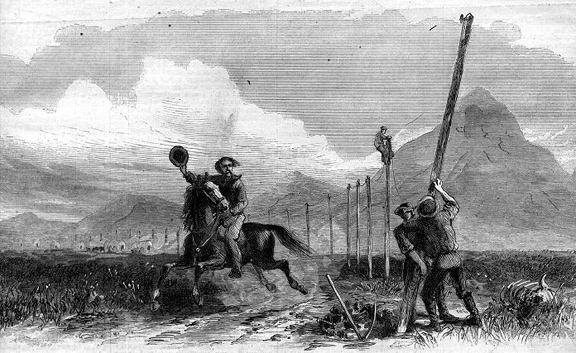
\includegraphics[width = 0.6\textwidth]{PoleA1}
        \caption{As primeiras linhas de telégrafo a serem construídas nos Estados Unidos \cite{polea1}.}
        \label{fig:polea1}
    \end{figure}
\end{frame}

\begin{frame}{Primeiro}
    
\end{frame}









\begin{frame}{História}
    \begin{figure}[ht]
        \begin{minipage}[b]{0.32\linewidth}
            \centering
            \includegraphics[width=\textwidth]{example-image}
            \caption{Label for a}
            \label{fig:3a}
        \end{minipage}
        \hspace{\fill}
        \begin{minipage}[b]{0.32\linewidth}
            \centering
            \includegraphics[width=\textwidth]{example-image}
            \caption{Label for b}
            \label{fig:3b}
        \end{minipage}
        \hspace{\fill}
        \begin{minipage}[b]{0.32\linewidth}
            \centering
            \includegraphics[width=\textwidth]{example-image}
            \caption{Label for c}
            \label{fig:3c}
        \end{minipage}
    \end{figure}
\end{frame}

\begin{frame}{História}
    \begin{figure}[ht]
        \begin{minipage}[b]{0.49\linewidth}
            \centering
            \includegraphics[width=\textwidth]{example-image}
            \caption{Label for a}
            \label{fig:2a}
        \end{minipage}
        \hspace{\fill}
        \begin{minipage}[b]{0.49\linewidth}
            \centering
            \includegraphics[width=\textwidth]{example-image}
            \caption{Label for b}
            \label{fig:2b}
        \end{minipage}
    \end{figure}
\end{frame}

\begin{frame}{Referências}
  \printbibliography
\end{frame}

\end{document}